\documentclass[border = 0.2cm]{standalone}

%\usetikzlibrary{...}% tikz package already loaded by 'tikz' option
\makeatletter
% Required packages and libraries
\usepackage {tikz}
\usetikzlibrary{arrows, automata}


\begin{document}

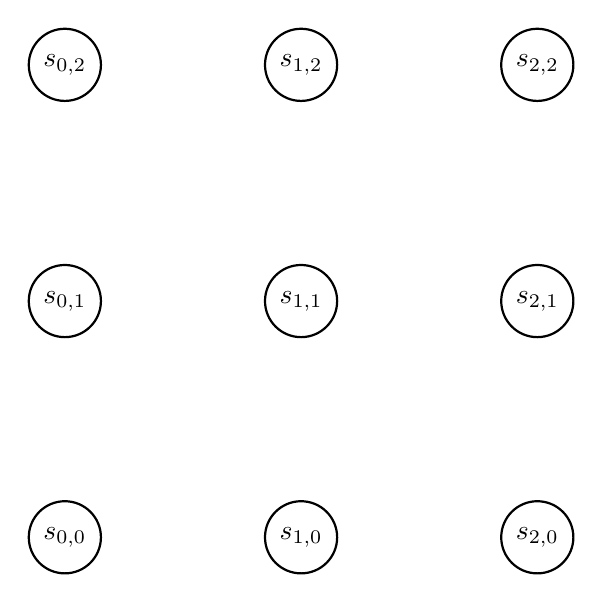
\begin{tikzpicture}[
            > = stealth, % arrow head style
            shorten > = 1pt, % don't touch arrow head to node
            auto,
            node distance = 3cm, % distance between nodes
            semithick % line style
        ]

        \tikzstyle{every state}=[
            draw = black,
            thick,
            fill = white,
            minimum size = 4mm
        ]

        \node[state] (s00) {$s_{0, 0}$};
        \node[state] (s10) [right of=s00] {$s_{1, 0}$};
        \node[state] (s20) [right of=s10] {$s_{2, 0}$};
        \node[state] (s01) [above of=s00] {$s_{0, 1}$};
        \node[state] (s11) [right of=s01] {$s_{1, 1}$};
        \node[state] (s21) [right of=s11] {$s_{2, 1}$};
        \node[state] (s02) [above of=s01] {$s_{0, 2}$};
        \node[state] (s12) [right of=s02] {$s_{1, 2}$};
        \node[state] (s22) [right of=s12] {$s_{2, 2}$};
        
    \end{tikzpicture}

\end{document}
